\section{Designing SimpleSpeech}
Building on the capabilities developed in these prior studies, SimpleSpeech is a web-based application for recording and editing short voice messages in a discussion setting.
Our user interface is quite similar to those created by Rubin \cite{rubin}, Yoon \cite{yoon}, and Whittaker \cite{whittaker_semantic}, which also provide lightweight audio editing capabilities.
Nevertheless, some slight conceptual modifications were necessary to suit the ``live'' editing paradigm, which we discuss below.
The appearance of the final SimpleSpeech user interface (UI) is shown in Fig. \ref{fig:overview_shot}.

We followed an iterative procedure to progressively improve the design and interactions of SimpleSpeech.
After building an initial prototype of the application, an informal pilot test was conducted with 5 participants (4 female, 1 male). 
Each user was given a brief introduction to the software and shown how to use the basic features, then given the scenario of creating an audio response to a written claim on an online forum. 
(The prompts used in the tests were adapted from the GRE Pool of Issue Topics.)
The user feedback helped us improve the capabilities of SimpleSpeech, including adding a transcript editing quasi-mode and enabling pause insertion.

Our text-based approach to speech editing requires a reliable transcription as well as time intervals corresponding to each word.
Both of these requirements are fulfilled by the IBM Watson Developer Cloud speech-to-text transcription service, which is reported to have a word error rate of 10.4\% \cite{soltau:2014}.

\red{I think that most of this paragraph about waveform, together with the Fig. \ref{fig:playback}, can be dropped. You can also drop any mention about waveform in the qualitative study, and the conclusion. Having waveform together is not a novel feature, nor the qualitative study users enjoyed it.} We chose to include a waveform visualization as part of the UI in order to remind the user that he or she is ultimately manipulating audio, not text. 
The waveform, as shown in Fig. \ref{fig:playback}, incorporates several subtle indications of the mapping between its contents and the transcription, including highlighting the audio corresponding to the current selection of tokens and animating deletions and insertions.
We found the presence of a waveform to be a helpful visual indicator of the purpose of SimpleSpeech because without it, users' inclination was to disregard the original speech and use the system as a dictation tool.

\red{Now the system description looks too flat without any punchlines. Here, I would like to have brief description about the three small new features: voice insertion at the cursor position, pause extension, and in-situ correction of transcription errors. AC wanted us to streamline the design section, so we don't have to present these three as NOVEL features. However, none of the reviewers argued against any of these features, so, presenting them will not hurt anybody. It's a simple balancing. Let's describe it without saying that these are novel. You can re-use some of old writing that you've deleted for this first revision.}

\begin{figure}
	\centering
	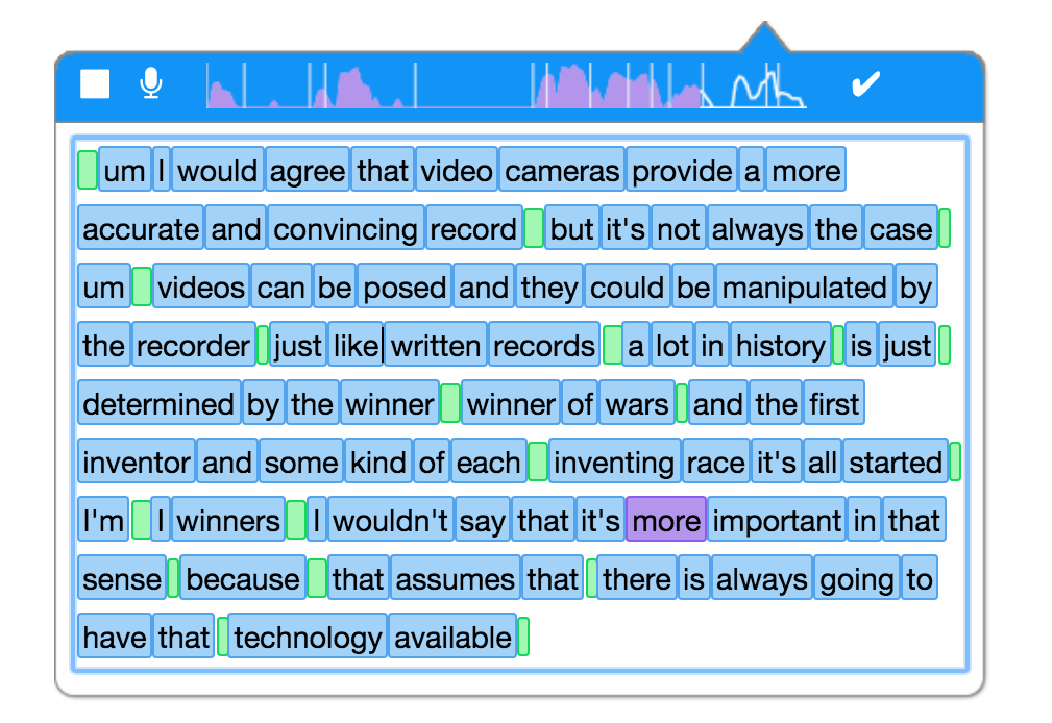
\includegraphics[width=\columnwidth,keepaspectratio]{figures/playback}
	\caption{The waveform visual at the top of the SimpleSpeech editor does not support direct millisecond-level editing; instead, it serves as a visual cue connecting the transcript to the working recording. For instance, the waveform is highlighted during playback in tandem with the current word that is being played.}~\label{fig:playback}
\end{figure}

Our use of text as a proxy for editing audio rendered it necessary to clearly delineate the capabilities of SimpleSpeech in comparison to a word processor.
However, we found the capability to edit text of individual words in the transcript to be desirable, especially in the case of ASR errors.
As shown in Fig. \ref{fig:transcription}, the transcription editing functionality is available in a separate mode, accessed by pressing the Return key.
The pop-up box insulates the editing within single words to avoid undermining the cohesiveness of the tokens. \red{I also acknowledge that you've described the 'in-situ correction' here. But I think the previous writing about Tokenization was much better as that tells 'why' we designed it that way. You can reuse that paragraph as well. But I will not re-use 'Playback shortcut', because one of the reviewer was against it explicitly "providing a shortcut is not design".}

\begin{figure}
	\centering
	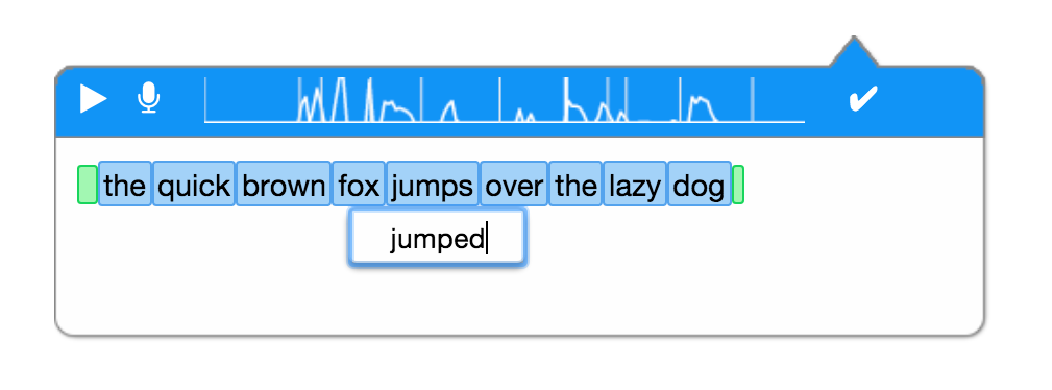
\includegraphics[width=\columnwidth,keepaspectratio]{figures/transcription_edit}
	\caption{To keep the user interface from becoming cluttered with secondary functionality, the transcription editing feature was implemented as a modal interaction. The pop-up box shown above ``opens'' the selected tokens for text editing in a separate control element, thus notifying the user that he or she is no longer directly editing the audio.}
	\label{fig:transcription}
\end{figure}